\documentclass[12pt]{article}



\usepackage{hyperref}

\usepackage[margin=1.25in]{geometry}
\usepackage{graphicx}
\graphicspath{ {./images/} }
\usepackage{imakeidx}
\makeindex[columns=3, title=Alphabetical Index, intoc]

\begin{document}

\begin{titlepage}

\title{%
  HW1: Mid-term assignment report\\
  \large  Testing and Software Quality\\}

\author{Rafael Remígio 102435}

\maketitle

\vfill
\begin{center}

	Departamento de Electrónica, Telecomunicações e Informática\\
       Universidade de Aveiro\\ Year 2022/2023
\end{center}



\end{titlepage}

\tableofcontents


\section{Introduction}

\subsection{Overview of the work} 


\subsection{Current limitations} 


\section{Product specification}


\subsection{Functional scope and supported interactions }

\subsection{System architecture}

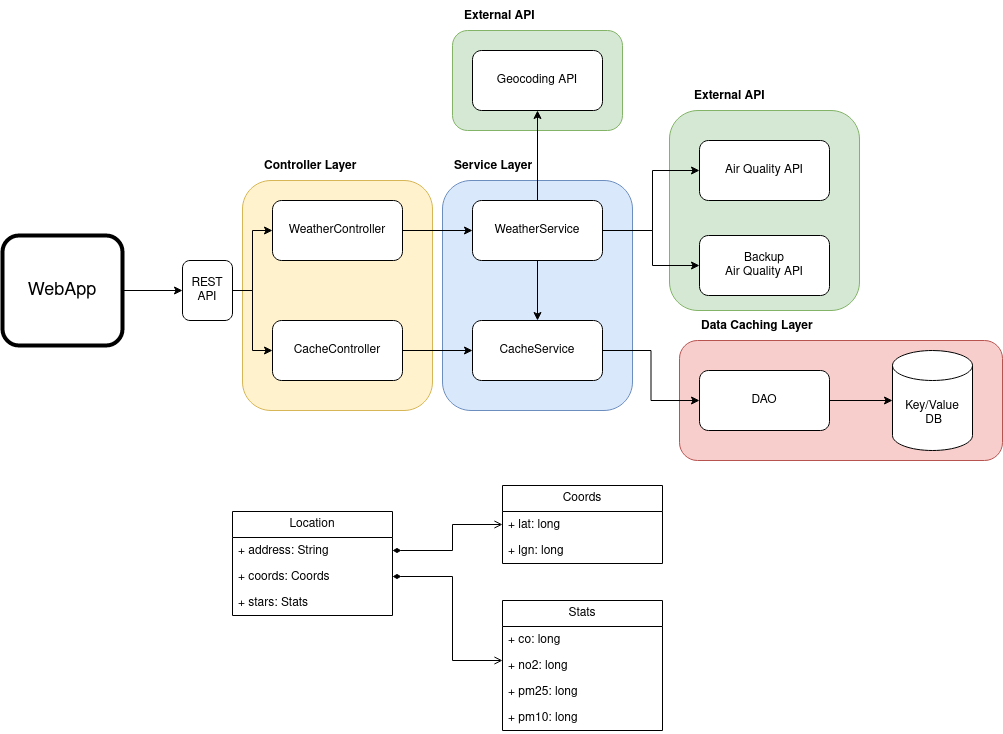
\includegraphics[scale=.4]{architecture.png}

\subsection{API for developers}

\section{Quality assurance}

\subsection{Overall strategy for testing}

\subsection{Unit and integration testing}

\subsection{Functional testing}

\subsection{Code quality analysis}

SonarQube

\subsection{Continuous integration pipeline}

\section{References \& resources}

GitRepository can be found at \"my github\".
\subsection{Reference materials}

\end{document}